\documentclass[04.3_buildingProcess.tex]{subfiles}
\begin{document}
    \subsubsection{Laser Cutting Process}
    \begin{flushleft}
        \noindent
        After milling the base, some experiments with a laser cutter was done. The distance between the
        cuts is essential for flexibility. To laser cut everything, Illustrator\cite{illustrator} and 
        Inkscape \cite{inkscape} and a laser cutter was used. With these programs, the shape can be 
        designed and can be uploaded on the cutter. \\~\\

        \noindent
        At first, acrylic glass has been cut because it is transparent and it would help to light up 
        a larger space; however, after a fail, wood was the second best choice. See the whole cutting process 
        in Figure \ref{fig:laserCutTests}

        \begin{figure}[H]
            \centering
            \begin{subfigure}{.45\textwidth}
            \centering
            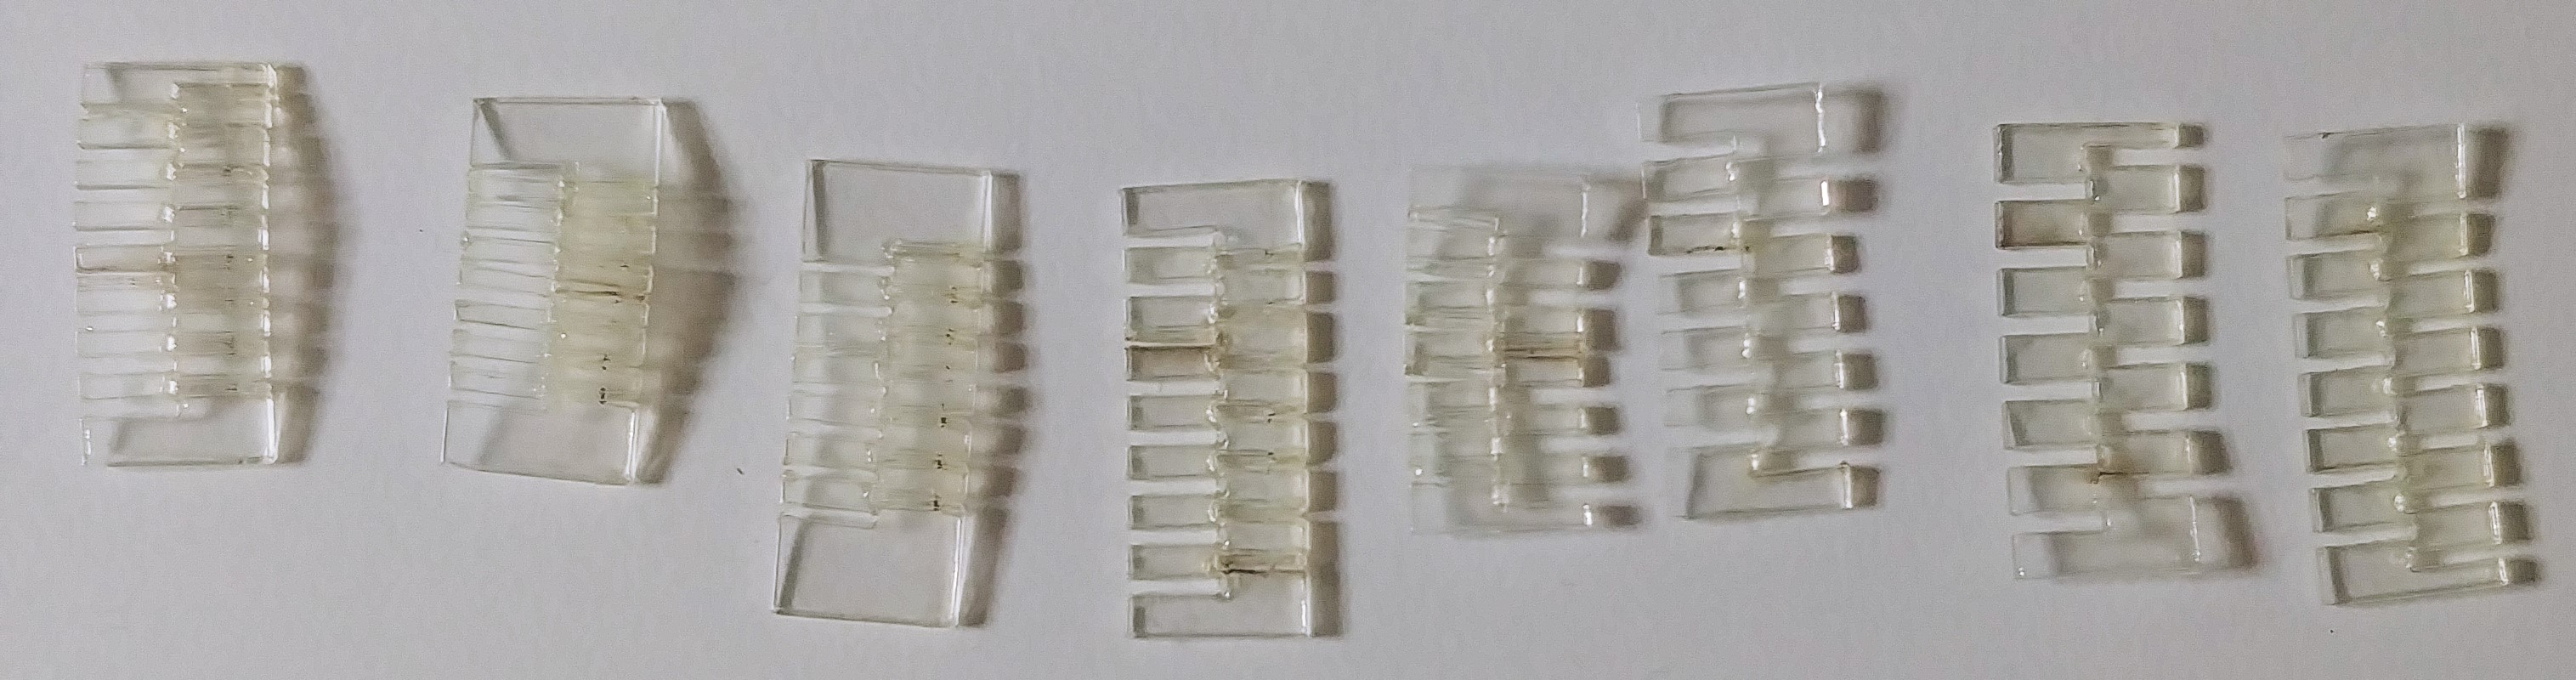
\includegraphics[width=0.8\linewidth]{images/materialProcess/01_LaserCut.jpg}
            \caption{Shows the first try to laser cut in general, so we wanted to
                    find out what distances of the wholes and how big the wholes 
                    should be in general.}
            \label{fig:01_LaserCut}
            \vspace{6mm}
            \end{subfigure}
            \medskip
            \hspace{1mm}
            \begin{subfigure}{.45\textwidth}
                \centering
                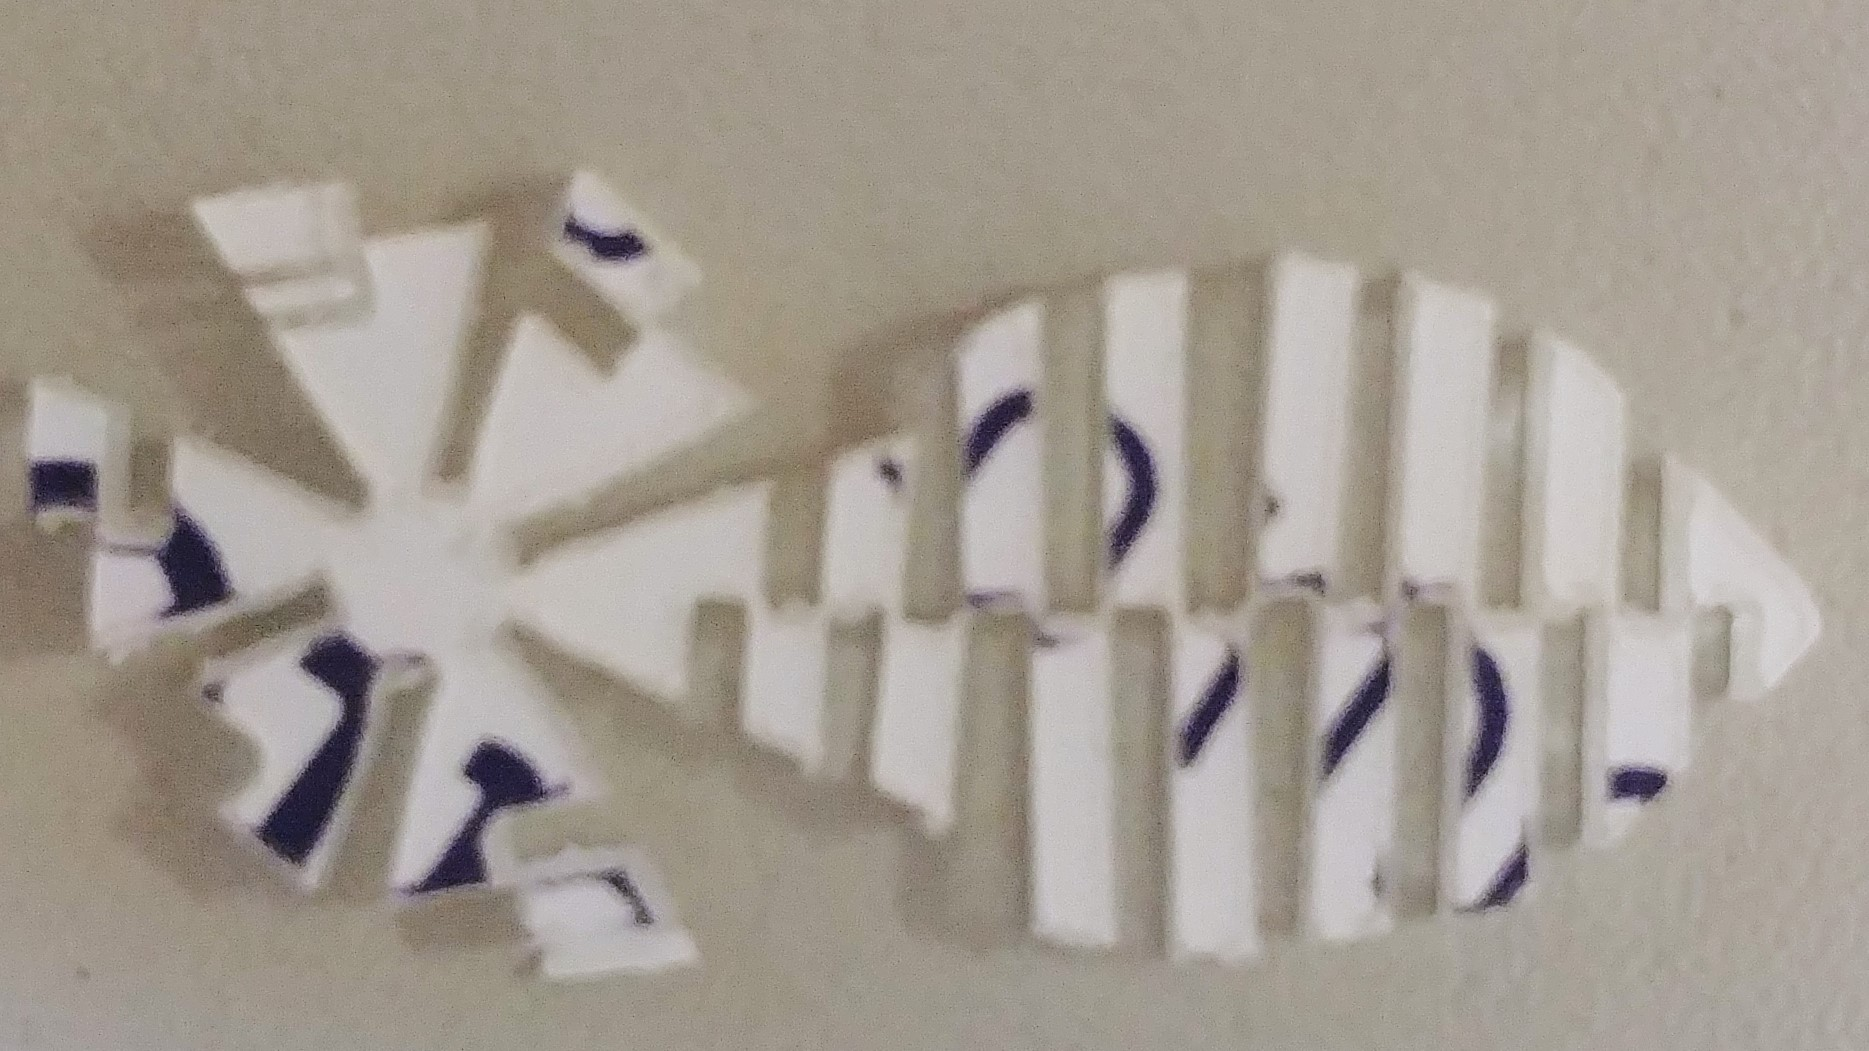
\includegraphics[width=0.8\linewidth]{images/materialProcess/02_LaserCut.jpg}
                \caption{Shows the second try to laser cut the shape. This time we have been
                        working with acrylic glass that was 2mm thin. The wholes are 1mm thick 
                        and the distance between those are only 5mm. When we tried to move
                        the parts, they broke.}
                \label{fig:02_LaserCut}
                \vspace{6mm}
            \end{subfigure}
            \hspace{1mm}
            \begin{subfigure}{.45\textwidth}
                \centering
                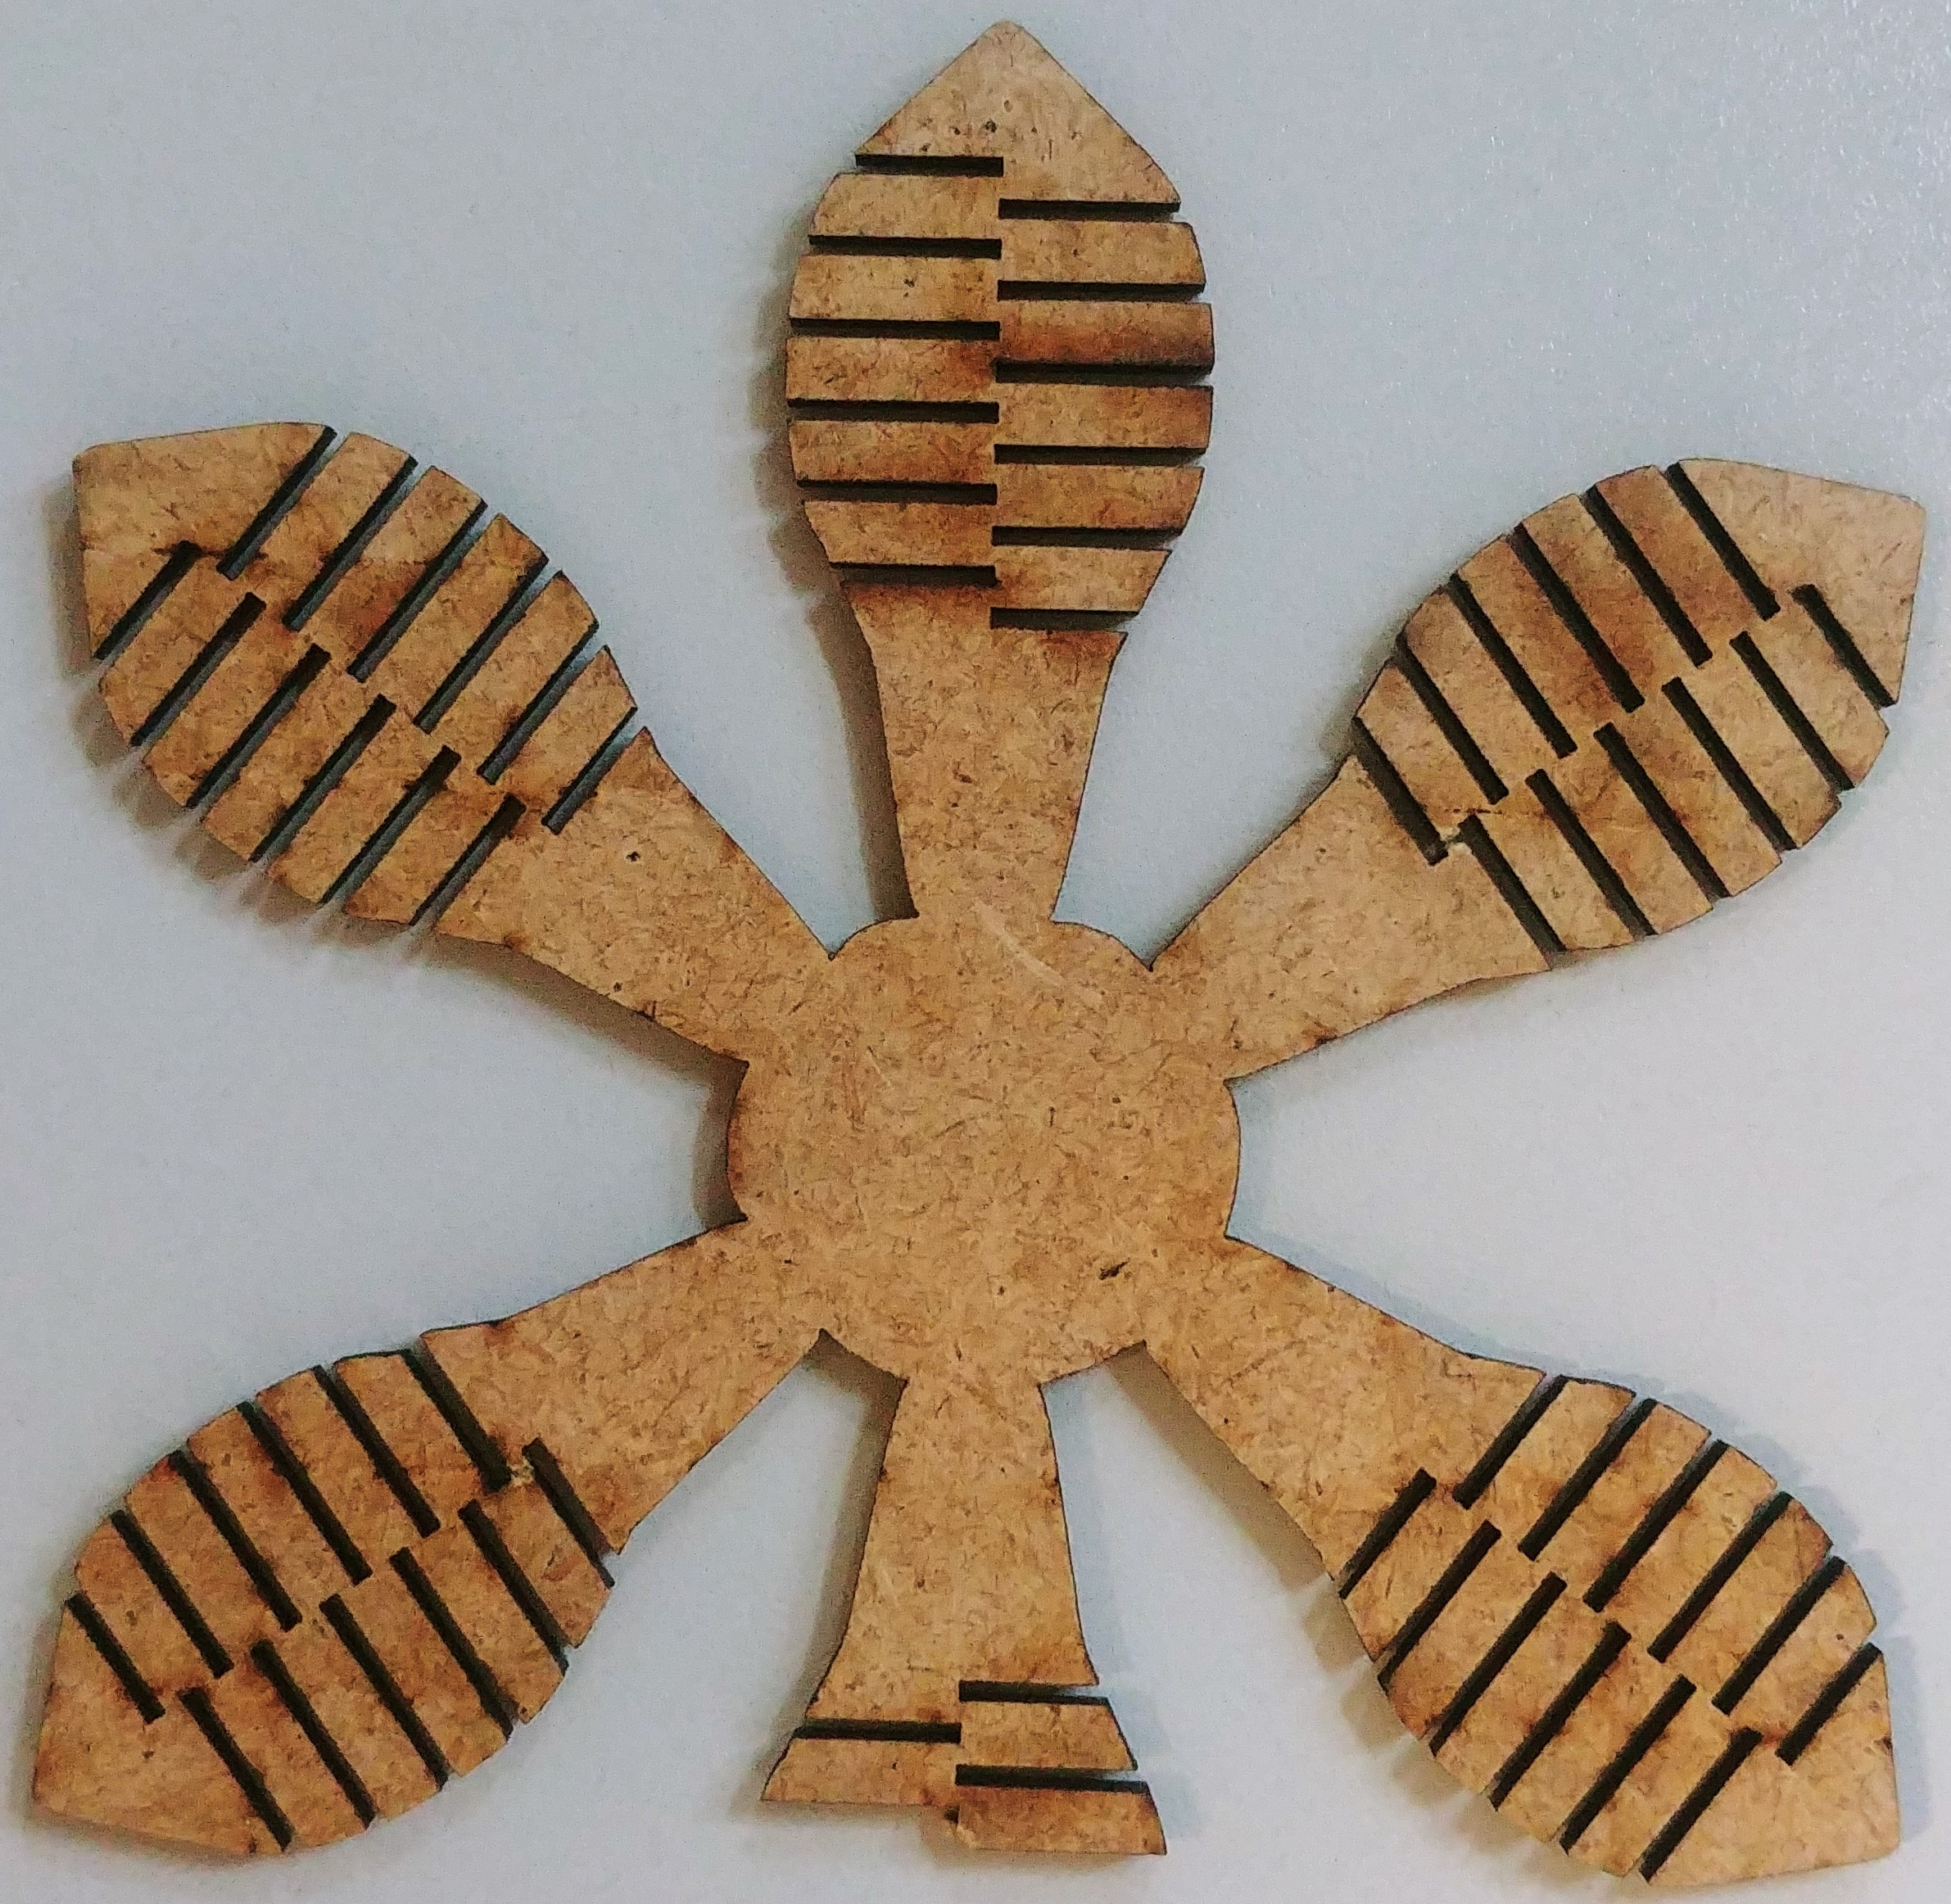
\includegraphics[width=0.6\linewidth]{images/materialProcess/03_LaserCut.jpg}
                \caption{Shows the third try to laser cut the shape. This time we have been
                        working with wood plate what is 3mm thin. The wholes are 1mm thick 
                        and the distance between those are only 5mm. When we tried to move
                        the parts, they broke.}
                \label{fig:03_LaserCut}
                \vspace{6mm}
            \end{subfigure}
            \hspace{1mm}
            \begin{subfigure}{.45\textwidth}
                \centering
                \includegraphics[width=0.77\linewidth]{images/materialProcess/04_LaserCut.jpg}
                \caption{Shows the fourth try to laser cut the shape. This time we have been
                        working with MDR 1mm thin plate. The wholes are 0.5mm thick and the 
                        distance between those are only 2.5mm, so they broke.}
                \label{fig:04_LaserCut}
                \vspace{6mm}
            \end{subfigure}
            \hspace{1mm}
            \begin{subfigure}{.45\textwidth}
                \centering
                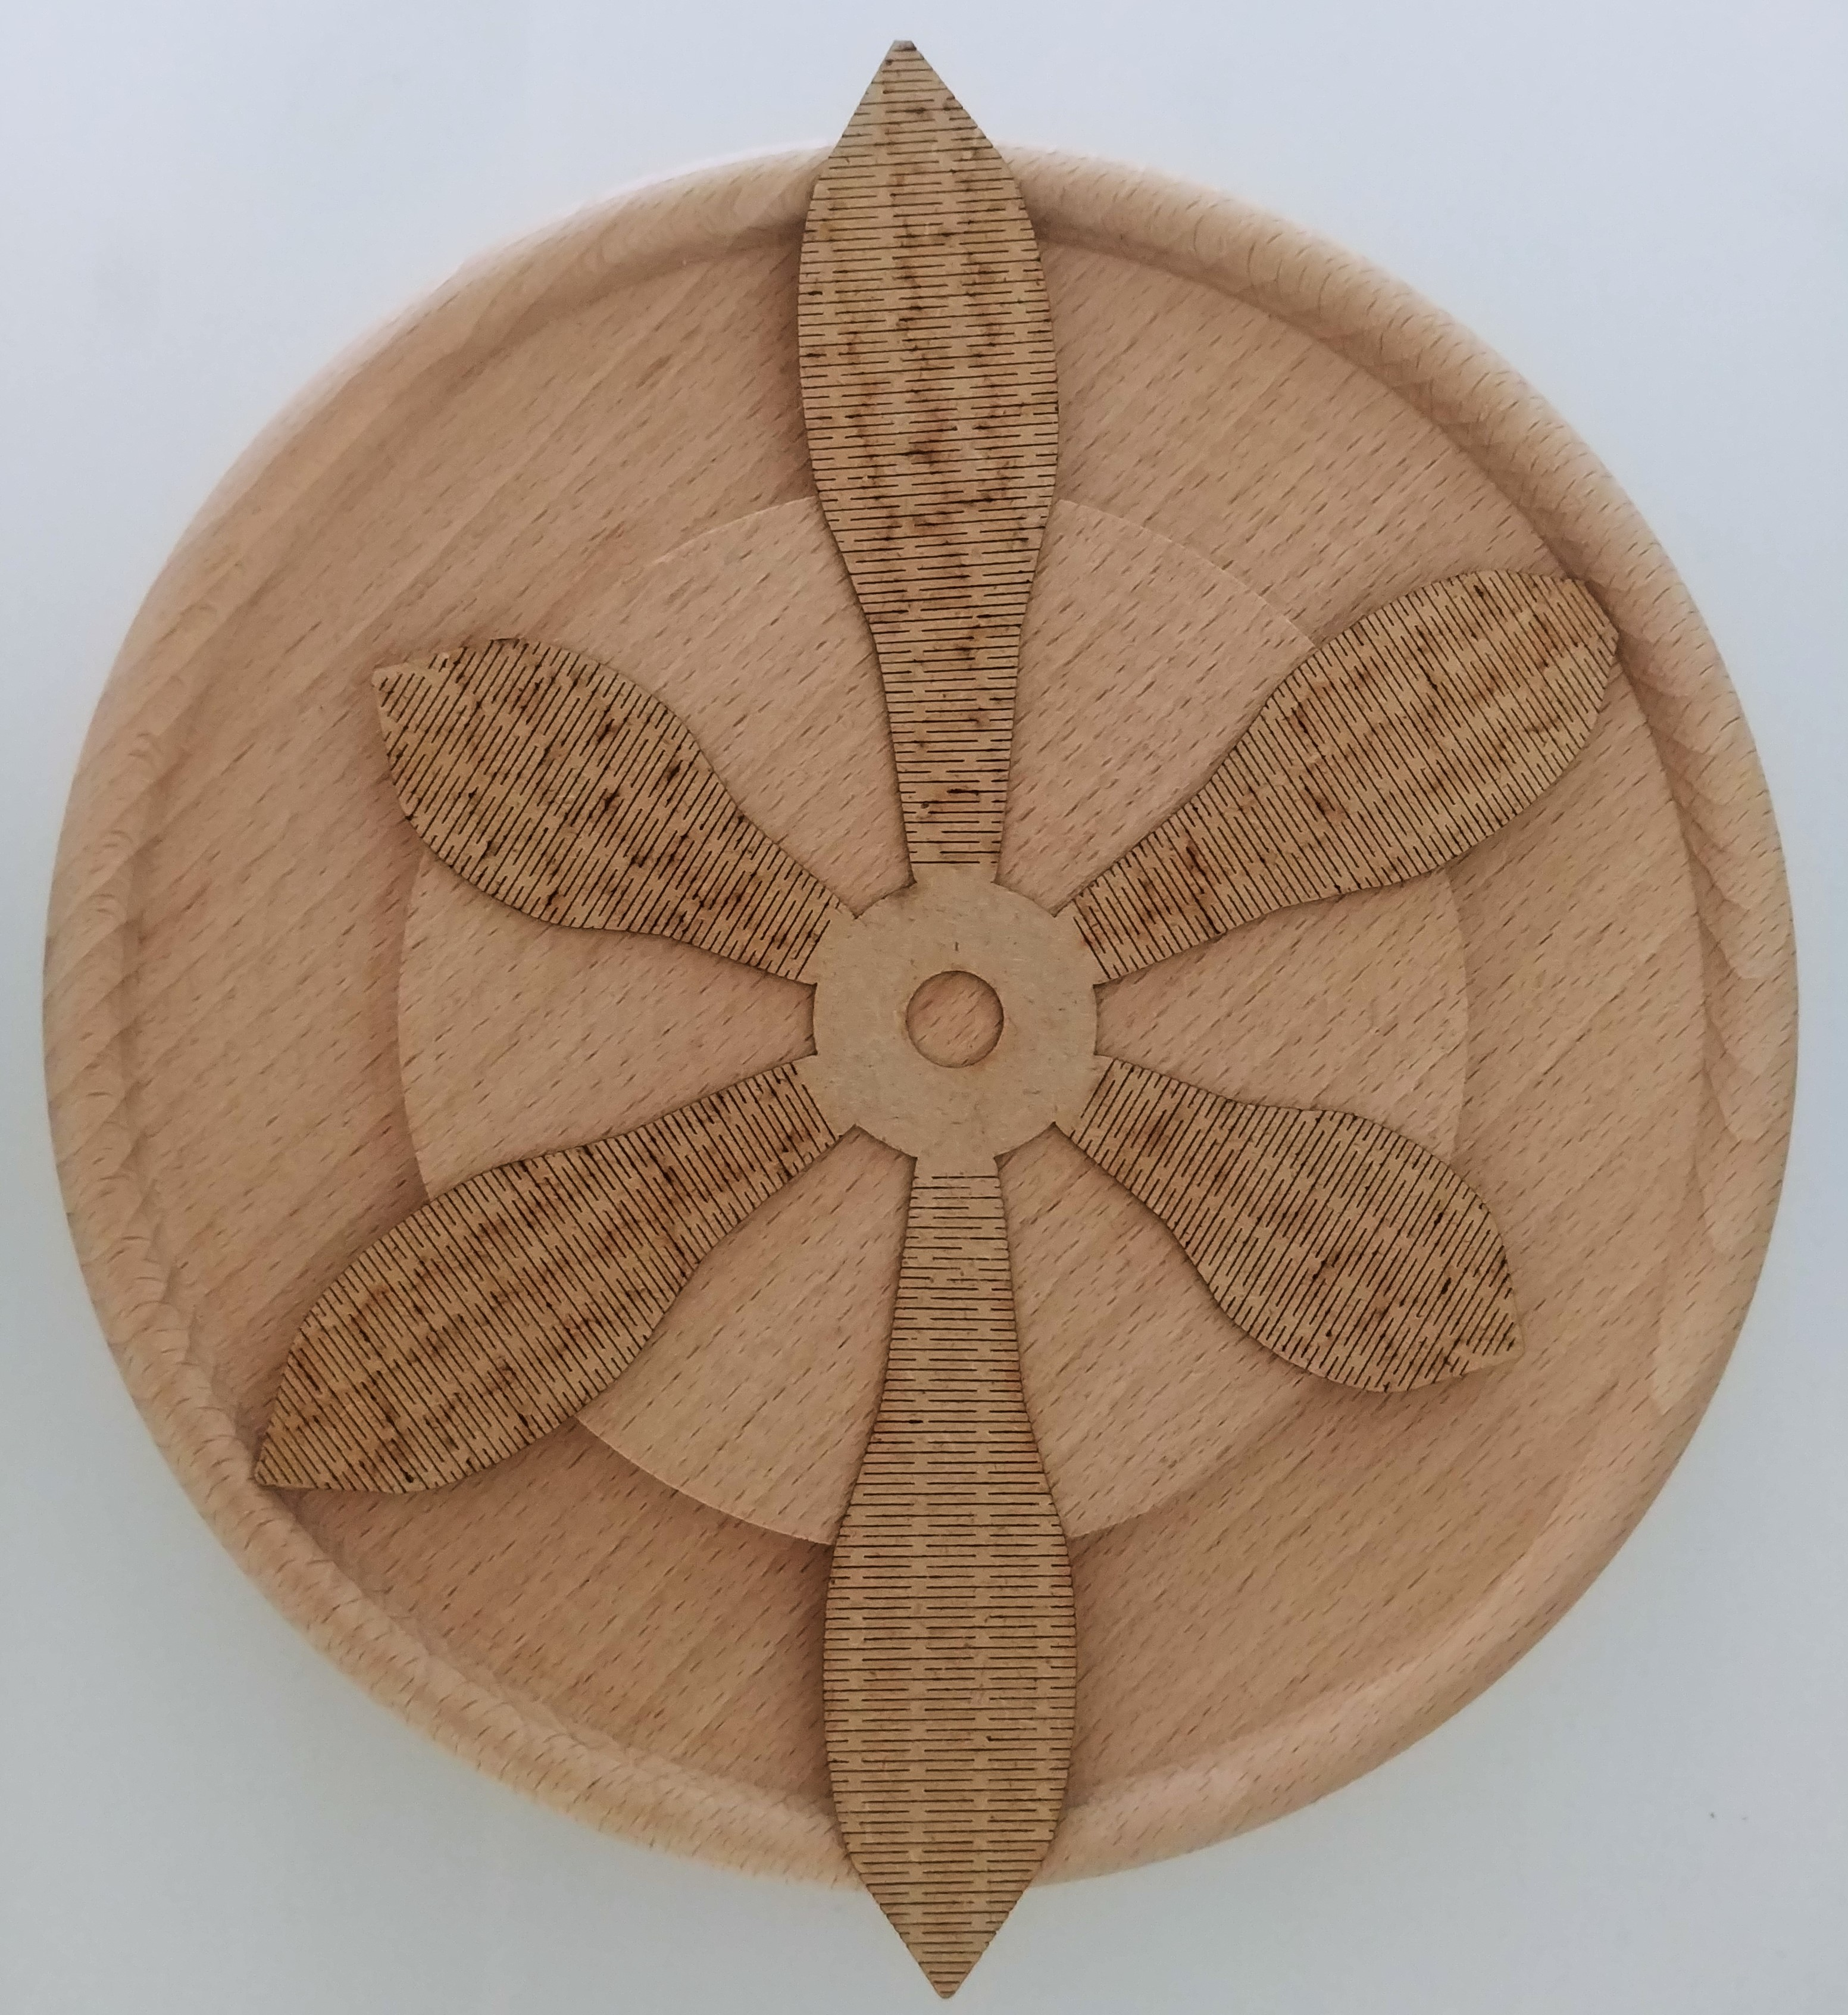
\includegraphics[width=0.6\linewidth]{images/materialProcess/06_LaserCut.jpg}
                \caption{Shows the sixth try with MDR 1mm thin plate.}
                \label{fig:04_LaserCut}
                \vspace{6mm}
            \end{subfigure}
            \begin{subfigure}{.45\textwidth}
                \centering
                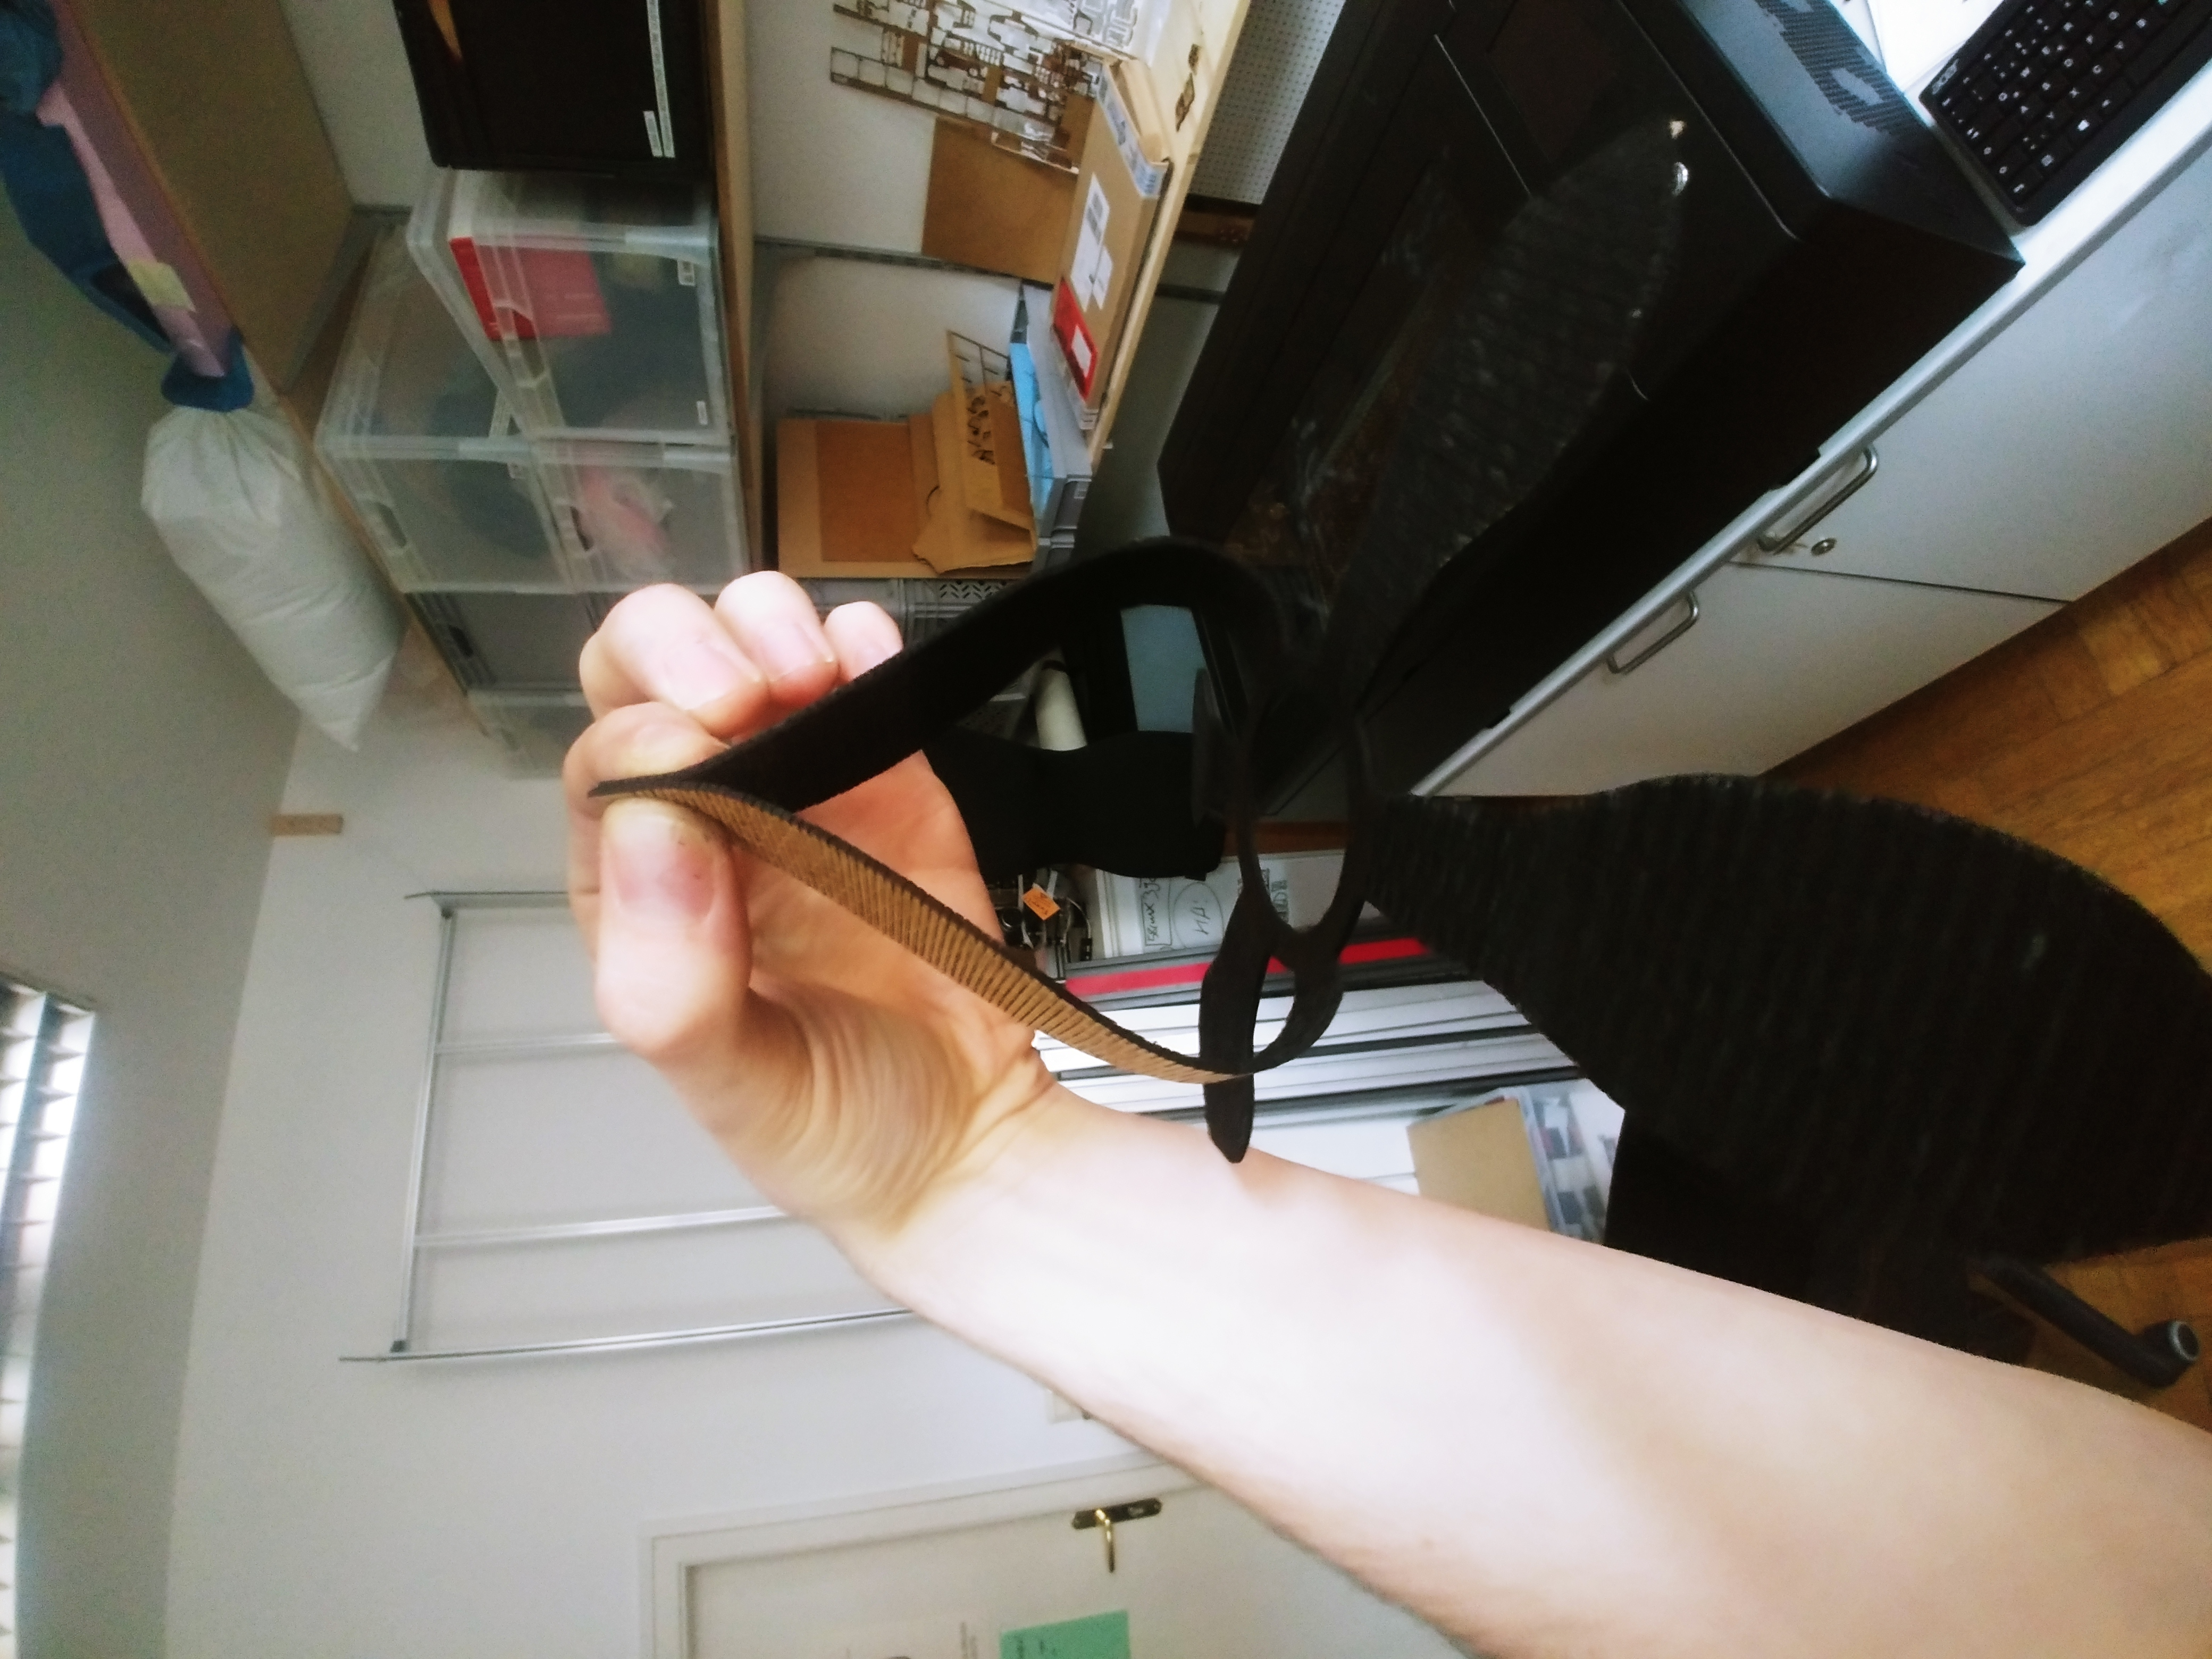
\includegraphics[width=0.65\linewidth, angle=270]{images/materialProcess/08_LaserCut.jpg}
                \caption{Shows the final laser cut that shows that it is flexiable.}
                \label{fig:08_LaserCut}
                \vspace{6mm}
            \end{subfigure}
            \caption{Shows the process of laser cuttings.}
            \label{fig:laserCutTests}
        \end{figure}
    \end{flushleft}
\end{document}